% =============================================================================
% CHAPTER 3: METHODOLOGY
% =============================================================================

\chapter{METHODOLOGY}
\label{Chapter3}

% -----------------------------------------------------------------------------
\section{Introduction}
\label{sec:ch3intro}
% -----------------------------------------------------------------------------

This chapter formalises the permissiveness problem identified in Chapter~2 and presents the Dynamic Context-Aware Trie (DCA-Trie) framework as a solution. The upgraded oracle specification and the Semantic Irrelevance Ratio (SIR) are defined first, with SIR serving as a diagnostic metric that measures constraint quality independently of answer accuracy. The chapter then traces the research evolution from an initial cosine-similarity scorer through a decomposed product score to the final symbolic TypeOracle, explaining why each earlier design was abandoned. The static pre-filtering design of v1 and the step-wise dynamic expansion design of v2 are described using the TypeOracle mechanism. The chapter closes with the baseline configurations, evaluation protocol, and scope boundaries that govern the experimental work in Chapter~4.

Unlike earlier embedding-based formulations, the final methodology implements semantic filtering through a deterministic TypeOracle. The TypeOracle uses the knowledge graph's own ontology metadata, especially entity types and relation ranges, instead of sentence-transformer embeddings, cosine similarity, or tuned admission thresholds.

% -----------------------------------------------------------------------------
\section{Formal Problem Specification}
\label{sec:ch3problem}
% -----------------------------------------------------------------------------

\subsection{Restating the Core Limitation of Existing Frameworks}

As established in Chapter~2, current graph-constrained frameworks (notably GCR \citep{luo2025-graph-constrained-reasoning} and DoG \citep{li2024-decoding-on-graphs}) rely on a deterministic oracle that looks only at the fixed graph $\mathcal{G}$ and the starting entities $\mathcal{E}_q$. Regardless of whether the system builds this oracle before decoding or expands it on the fly, the set of valid tokens at any step $t$ remains locked to structural logic:
\begin{equation}
  \mathcal{W}_{\text{val}}^{\text{GCR}}(t) = f(\mathcal{G},\, \mathcal{E}_q)
  \quad \forall\, t
  \label{eq:gcr_oracle}
\end{equation}

Equation~\eqref{eq:gcr_oracle} captures this static constraint model. By ignoring both the semantic intent of the question $q$ and the reasoning trajectory already captured in the prefix $y_{<t}$, this formulation treats every structurally reachable path as equally plausible. In dense, multi-hop Freebase environments, this causes substantial search space inflation. The oracle can admit over 8,000 paths at depth 3, even though only a single path logically answers the query.

Two separate requirements are in tension here. Structural validity ensures the LLM only generates tokens that correspond to real graph edges; current models do this well. Contextual relevance is the open problem: ensuring the LLM only generates tokens that logically connect to the specific question. Current models do not enforce this. The gap between structural compliance and semantic usefulness is the \textit{permissiveness problem}.

\subsection{The Upgraded Oracle Specification}

DCA-Trie addresses this problem by defining a constraint oracle that conditions on both the input question and the evolving generation prefix:
\begin{equation}
  \mathcal{W}_{\text{val}}^{\text{DCA}}(t) = f(\mathcal{G},\, \mathcal{E}_q,\,
  q,\, y_{<t})
  \label{eq:dca_oracle}
\end{equation}
where $q$ is the natural language query and $y_{<t} = (y_1, \ldots, y_{t-1})$ is the generated prefix at step $t$. The upgraded oracle must satisfy three conditions aligned with the project objectives in Chapter~1:

\begin{enumerate}
  \item \textbf{Structural Faithfulness (Condition~F):} Every candidate token $v \in \mathcal{W}_{\text{val}}^{\text{DCA}}(t)$ must correspond to a valid prefix of a path $p \in \mathcal{G}$ at every step $t$. This preserves the 100\% structural faithfulness guarantee achieved by GCR and DoG and prevents ungrounded tokens from entering the valid set.

  \item \textbf{Semantic Relevance Reduction (Condition~R):} The Semantic Irrelevance Ratio (SIR) under DCA-Trie must be lower than the corresponding SIR under GCR when averaged over the evaluation corpus. Using SIR as defined in Section~\ref{sec:ch3sir}:
        \begin{equation}
          \overline{\text{SIR}}\!\left(\mathcal{W}^{\text{DCA}}\right) <
          \overline{\text{SIR}}\!\left(\mathcal{W}^{\text{GCR}}\right)
          \label{eq:sir_condition}
        \end{equation}

  \item \textbf{Recall Preservation (Condition~P):} Semantic pruning must not remove gold paths excessively. Operationally, the false negative rate (FNR) on the WebQSP validation split must remain below 5\%, as formalised in Equation~\eqref{eq:fnr}:
        \begin{equation}
          \text{FNR} = \frac{|\{q \in \mathcal{Q}_{\text{val}} :
            p^*_q \notin \mathcal{W}_{\text{val}}^{\text{DCA}}(t)\}|}{|\mathcal{Q}_{\text{val}}|}
          < 0.05
          \label{eq:fnr}
        \end{equation}
        where $p^*_q$ is the gold path for question $q$ and $\mathcal{Q}_{\text{val}}$ is the held-out 100-question validation set.

        These three conditions are not guaranteed to be jointly satisfiable. Tightening the oracle to satisfy Condition~R (reduce irrelevance) can directly threaten Condition~P (remove gold paths) when the semantic signal mismatches the lexical form of correct answers. This tension is the central axis of the Chapter~4 results.
\end{enumerate}


% -----------------------------------------------------------------------------
\section{System Architecture Overview}
\label{sec:ch3arch}
% -----------------------------------------------------------------------------

DCA-Trie focuses on the constraint oracle layer, so its architecture directly builds on the baseline pipeline from Graph-Constrained Reasoning (GCR) \citep{luo2025-graph-constrained-reasoning}. This reuse helps isolate the experimental effects of the proposed oracle. The four layers work as follows:

\begin{enumerate}
  \item \textbf{Entity Linking Layer (Unmodified):} A named entity recognition or entity-linking component identifies the core query entities $\mathcal{E}_q$ from the raw natural language question $q$. These entities dictate where downstream graph exploration begins.

  \item \textbf{Constraint Oracle Layer (DCA-Trie Contribution):} This layer controls which tokens the LLM can generate. In GCR, this layer creates a KG-Trie that includes structurally reachable paths within $L$ hops of the starting entities. DCA-Trie modifies this layer by applying symbolic ontology checks through a TypeOracle. Through either static pre-filtering (v1) or dynamic step-wise expansion (v2), the oracle ensures that admitted paths remain graph-valid and type-consistent.

  \item \textbf{Constrained Decoding Layer (Unmodified):} During autoregressive generation, the decoding layer intercepts the LLM logit distribution and applies a binary mask retrieved from the oracle layer. The LLM is therefore restricted to tokens that are currently valid under the trie.

  \item \textbf{Inductive Reasoning Layer (Unmodified):} After constrained decoding produces candidate reasoning paths, the answer synthesis component analyses these paths and produces the final natural language answer.
\end{enumerate}

Figure~\ref{fig:architecture} shows the full pipeline, isolating the constraint oracle layer to emphasise where the core symbolic intervention takes place. The TypeOracle box performs two deterministic set operations (range gate and type gate) rather than cosine scoring or embedding comparisons.

\begin{sidewaysfigure}[p]
  \centering
  \resizebox{\textwidth}{!}{%
    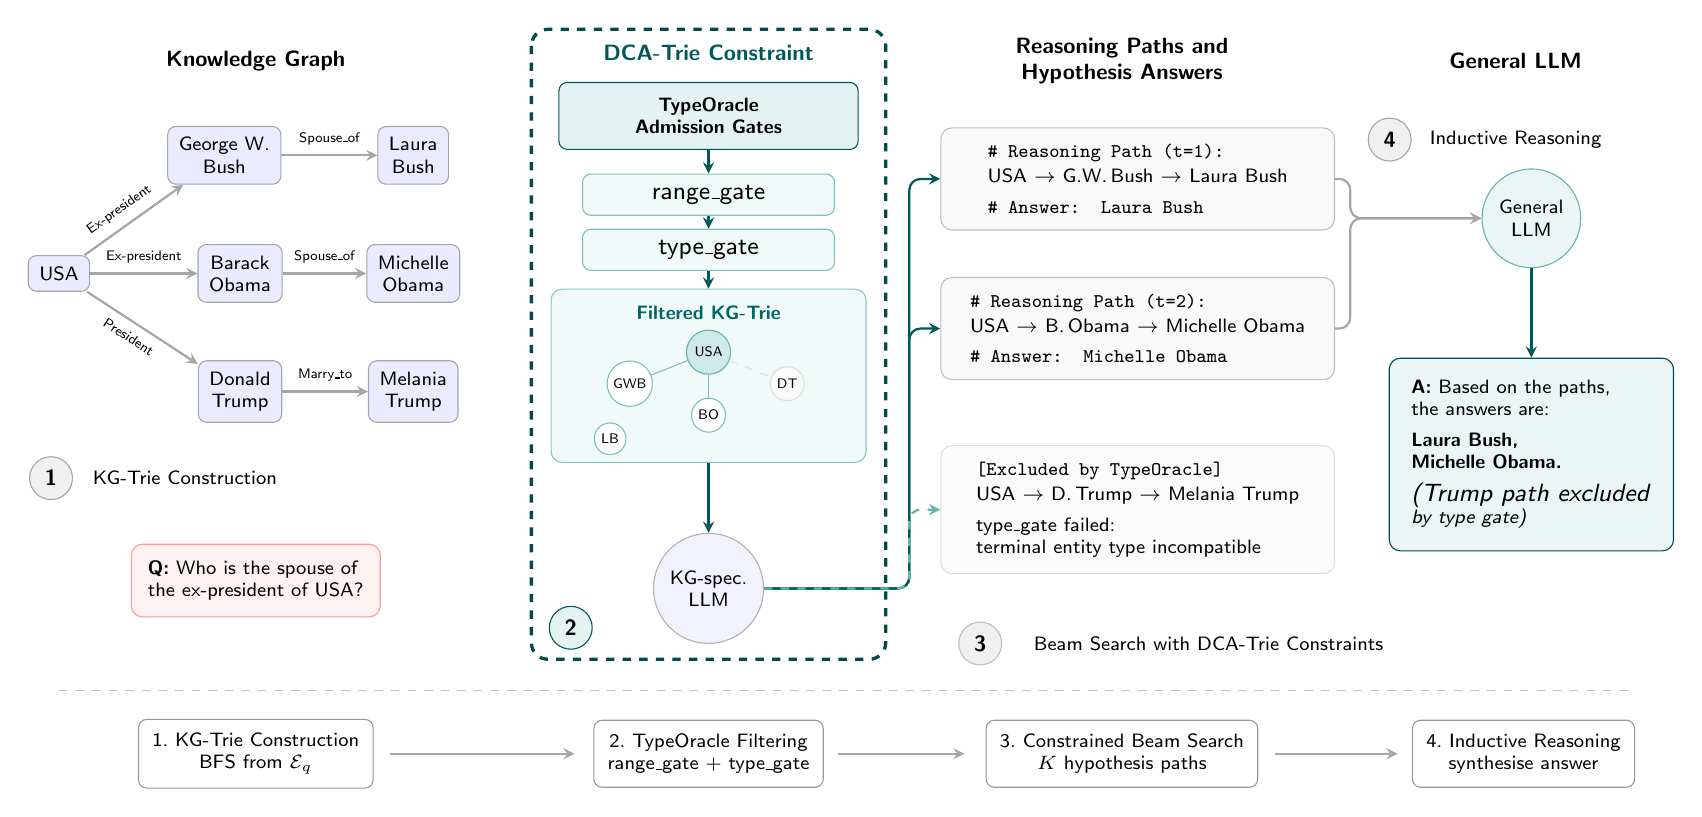
\begin{tikzpicture}[
        >=stealth, font=\sffamily,
        kgnode/.style={draw=gray!70,fill=blue!8,rounded corners=3pt,inner sep=4pt,font=\sffamily\scriptsize,align=center},
        pathbox/.style={draw=gray!50,fill=gray!5,rounded corners=4pt,inner sep=6pt,minimum width=5.0cm,align=left,font=\sffamily\scriptsize},
        ansbox/.style={draw=teal!60!black,fill=teal!8,rounded corners=4pt,inner sep=8pt,minimum width=3.0cm,align=left,font=\sffamily\scriptsize},
        stepbox/.style={draw=black!40,fill=white,rounded corners=3pt,inner sep=5pt,minimum width=2.6cm,minimum height=0.85cm,align=center,font=\sffamily\scriptsize},
        dcabox/.style={draw=teal!70!black,fill=teal!10,rounded corners=3pt,inner sep=5pt,minimum width=2.6cm,minimum height=0.85cm,align=center,font=\sffamily\scriptsize\bfseries},
        gatebox/.style={draw=teal!50,fill=teal!5,rounded corners=3pt,inner sep=4pt,font=\sffamily\small,align=center},
        llmcirc/.style={circle,draw=gray!60,fill=blue!5,minimum size=1.1cm,align=center,font=\sffamily\scriptsize},
        bigllm/.style={circle,draw=teal!60,fill=teal!8,minimum size=1.25cm,align=center,font=\sffamily\scriptsize},
        arr/.style={->,thick,draw=gray!70},
        tarr/.style={->,thick,draw=teal!70!black},
      ]

      % Knowledge Graph Section
      \node[font=\sffamily\footnotesize\bfseries]at(2.5,0.2){Knowledge Graph};
      \node[kgnode](usa)at(0,-2.5){USA};
      \node[kgnode](gwb)at(2.1,-1.0){George W.\\Bush};
      \node[kgnode](lb)at(4.5,-1.0){Laura\\Bush};
      \node[kgnode](bo)at(2.3,-2.5){Barack\\Obama};
      \node[kgnode](mo)at(4.5,-2.5){Michelle\\Obama};
      \node[kgnode](dt)at(2.3,-4.0){Donald\\Trump};
      \node[kgnode](mt)at(4.5,-4.0){Melania\\Trump};

      \draw[arr](usa)--node[above,sloped,font=\sffamily\tiny,pos=0.45]{Ex-president}(gwb);
      \draw[arr](usa)--node[above,font=\sffamily\tiny,pos=0.5]{Ex-president}(bo);
      \draw[arr](usa)--node[below,sloped,font=\sffamily\tiny,pos=0.45]{President}(dt);
      \draw[arr](gwb)--node[above,font=\sffamily\tiny]{Spouse\_of}(lb);
      \draw[arr](bo)--node[above,font=\sffamily\tiny]{Spouse\_of}(mo);
      \draw[arr](dt)--node[above,font=\sffamily\tiny]{Marry\_to}(mt);

      \node[draw=red!40,fill=red!5,rounded corners=4pt,inner sep=6pt,align=left,
        font=\sffamily\scriptsize,minimum width=2.9cm]
      (qbox)at(2.5,-6.4){\textbf{Q:} Who is the spouse of\\the ex-president of USA?};
      \node[circle,draw=black!35,fill=black!6,font=\sffamily\footnotesize\bfseries,inner sep=3pt]at(-0.1,-5.1){1};
      \node[font=\sffamily\scriptsize,text=black,align=center]at(1.6,-5.1){KG-Trie Construction};

      % DCA-Trie Constraint Section
      \draw[draw=teal!60!black,dashed,rounded corners=6pt,line width=1.2pt](6.0,0.6)rectangle(10.5,-7.4);
      \node[font=\sffamily\footnotesize\bfseries,text=teal!70!black]at(8.25,0.3){DCA-Trie Constraint};
      \node[dcabox,minimum width=3.8cm](vf)at(8.25,-0.5){TypeOracle\\Admission Gates};

      % TypeOracle gates inside the box
      \node[gatebox,minimum width=3.2cm](rg)at(8.25,-1.5){range\_gate};
      \node[gatebox,minimum width=3.2cm](tg)at(8.25,-2.2){type\_gate};

      \node[draw=teal!45,fill=teal!5,rounded corners=4pt,minimum width=4.0cm,minimum height=2.2cm](triebox)at(8.25,-3.8){};
      \node[font=\sffamily\scriptsize\bfseries,text=teal!80!black]at(8.25,-3.0){Filtered KG-Trie};

      \node[circle,draw=teal!60,fill=teal!18,inner sep=2pt,font=\sffamily\tiny](tr)at(8.25,-3.5){USA};
      \node[circle,draw=teal!50,fill=white,inner sep=1.5pt,font=\sffamily\tiny](tn1)at(7.25,-3.9){GWB};
      \node[circle,draw=teal!50,fill=white,inner sep=1.5pt,font=\sffamily\tiny](tn2)at(8.25,-4.3){BO};
      \node[circle,draw=gray!25,fill=gray!4,inner sep=1.5pt,font=\sffamily\tiny,text=black](tn3)at(9.25,-3.9){DT};
      \node[circle,draw=teal!50,fill=white,inner sep=1.5pt,font=\sffamily\tiny](tl1)at(7.0,-4.6){LB};


      \draw[teal!50,thin](tr)--(tn1); \draw[teal!50,thin](tr)--(tn2);
      \draw[gray!25,thin,dashed](tr)--(tn3);

      \node[llmcirc](kgllm)at(8.25,-6.5){KG-spec.\\LLM};

      \draw[tarr](vf)--(rg);
      \draw[tarr](rg)--(tg);
      \draw[tarr](tg)--(triebox.north);
      \draw[tarr](triebox.south)--(kgllm);

      \node[circle,draw=teal!70!black,fill=teal!10,font=\sffamily\footnotesize\bfseries,inner sep=3pt]at(6.5,-7){2};

      % Reasoning Paths and Hypothesis Answers Section
      \node[font=\sffamily\footnotesize\bfseries,align=center]at(13.5,0.2){Reasoning Paths and\\Hypothesis Answers};
      \node[circle,draw=black!25,fill=black!6,font=\sffamily\footnotesize\bfseries,inner sep=3pt]at(11.7,-7.2){3};
      \node[font=\sffamily\scriptsize,text=black]at(14.6,-7.2){Beam Search with DCA-Trie Constraints};
      \node[pathbox](p1)at(13.7,-1.3){%
        \texttt{\# Reasoning Path (t=1):}\\[1pt]
        USA $\to$ G.W.\,Bush $\to$ Laura Bush\\[3pt]
        \texttt{\# Answer: Laura Bush}};
      \node[pathbox](p2)at(13.7,-3.2){%
        \texttt{\# Reasoning Path (t=2):}\\[1pt]
        USA $\to$ B.\,Obama $\to$ Michelle Obama\\[3pt]
        \texttt{\# Answer: Michelle Obama}};
      \node[pathbox,draw=gray!25,fill=gray!3,text=black](p3)at(13.7,-5.5){%
        \texttt{[Excluded by TypeOracle]}\\[1pt]
        USA $\to$ D.\,Trump $\to$ Melania Trump\\[3pt]
        type\_gate failed:\\
        terminal entity type incompatible};

      \draw[tarr,rounded corners](kgllm.east)-- (10.8,-6.5) |- (p1.west);
      \draw[tarr,rounded corners](kgllm.east)-- (10.8,-6.5) |- (p2.west);
      \draw[tarr,dashed,draw=teal!60,rounded corners](kgllm.east)-- (10.8,-6.5) |- (p3.west);

      % General LLM Section
      \node[font=\sffamily\footnotesize\bfseries]at(18.5,0.2){General LLM};
      \node[bigllm](gllm)at(18.7,-1.8){General\\LLM};
      \node[ansbox](ans)at(18.7,-4.8){%
        \textbf{A:} Based on the paths,\\
        the answers are:\\[3pt]
        \textbf{Laura Bush,}\\
        \textbf{Michelle Obama.}\\[4pt]
        \small\textit{(Trump path excluded}\\
        \textit{by type gate)}};
      \node[circle,draw=black!35,fill=black!6,font=\sffamily\footnotesize\bfseries,inner sep=3pt]at(16.9,-0.8){4};
      \node[font=\sffamily\scriptsize,text=black]at(18.5,-0.8){Inductive Reasoning};

      \draw[arr,rounded corners](p1.east) -| (16.4,-1.8) -- (gllm.west);
      \draw[arr,rounded corners](p2.east) -| (16.4,-1.8) -- (gllm.west);
      \draw[tarr](gllm)--(ans);

      % Footer Steps Section
      \draw[gray!50,dashed](0,-7.8)--(20.0,-7.8);
      \node[stepbox]at(2.5,-8.6){1.\ KG-Trie Construction\\BFS from $\mathcal{E}_q$};
      \node[stepbox]at(8.25,-8.6){2.\ TypeOracle Filtering\\range\_gate + type\_gate};
      \node[stepbox]at(13.5,-8.6){3.\ Constrained Beam Search\\$K$ hypothesis paths};
      \node[stepbox]at(18.6,-8.6){4.\ Inductive Reasoning\\synthesise answer};

      \draw[arr](4.2,-8.6)--(6.55,-8.6);
      \draw[arr](9.9,-8.6)--(11.5,-8.6);
      \draw[arr](15.45,-8.6)--(17.0,-8.6);
    \end{tikzpicture}
  }%
  \caption[DCA-Trie System Architecture]{DCA-Trie System Architecture.}
  \label{fig:architecture}
\end{sidewaysfigure}

% -----------------------------------------------------------------------------
\section{The Semantic Irrelevance Ratio: Definition and Measurement}
\label{sec:ch3sir}
% -----------------------------------------------------------------------------

\subsection{Standard Metric Deficiencies}

Current performance markers for knowledge graph decoding, such as Hits@1, F1, and structural faithfulness ratios, have a significant drawback: they focus on output instead of the process. While these metrics show whether a framework found the correct answer and stayed within the graph, they do not reveal how the framework reached that answer. A model may solve the correct gold path, but it could wander through a large number of irrelevant paths that waste resources.

Confirming accuracy is not enough; the constraint mechanism itself must be measured. To assess how permissive the oracle is, independently of final answer accuracy, this thesis presents a diagnostic metric called the Semantic Irrelevance Ratio (SIR).

\subsection{Formal Definition of SIR}

Suppose $\mathcal{P}(q, t)$ represents all paths that the constraint oracle allows at decoding step $t$ for question $q$. To calculate SIR, the system must first define irrelevance. An individual candidate path $p \in \mathcal{P}(q, t)$ is structurally valid, but it fails the semantic stringency test if its terminal entity type is incompatible with the inferred answer types, or if any edge in the path violates the property range constraint:
\begin{equation}
  \text{irrelevant}(p, q) = \mathbf{1}\!\left[
    \neg\,\text{type\_gate}(p, q) \;\lor\;
    \exists\, (e, r, e') \in p :
    \neg\,\text{range\_gate}(r, e')
    \right]
  \label{eq:irrelevant}
\end{equation}
Equation~\eqref{eq:irrelevant} defines the binary irrelevance indicator. Here, type\_gate checks whether the terminal entity's type matches the expected answer types inferred from the question, and range\_gate checks whether each edge respects the ontology's declared property ranges. Both gates are deterministic set operations over the KG's own schema, defined in Section~\ref{sec:ch3oracle}.

The step-level SIR for question $q$ at decoding step $t$ is then defined as:
\begin{equation}
  \text{SIR}(q, t) = \frac{\sum_{p \in \mathcal{P}(q,t)}
    \text{irrelevant}(p, q)}{|\mathcal{P}(q, t)|}
  \label{eq:sir_step}
\end{equation}
As shown in Equation~\eqref{eq:sir_step}, this quantity is the fraction of admitted paths at step $t$ that are semantically irrelevant.

Corpus-level SIR is computed by averaging over all questions and all valid decoding steps up to depth $L$:
\begin{equation}
  \overline{\text{SIR}} = \frac{1}{|\mathcal{Q}|} \sum_{q \in \mathcal{Q}}
  \frac{1}{L_q} \sum_{t=1}^{L_q} \text{SIR}(q, t)
  \label{eq:sir_aggregate}
\end{equation}
Equation~\eqref{eq:sir_aggregate} gives the corpus-level average, where $L_q$ is the hop length of the generated reasoning chain for question $q$.

\subsection{Properties and Interpretation}

By definition, $\overline{\text{SIR}} \in [0,1]$. A value near 1 indicates that most admitted paths are irrelevant, so the model still faces a large and noisy search space. A value near 0 indicates that the constraint set is tightly aligned with question semantics. Prior constrained frameworks such as GCR and DoG tend to show high SIR, especially at larger hop depths where path counts increase rapidly. DCA-Trie targets lower SIR by filtering semantically weak paths. The structurally valid ones stay. In reporting, SIR is analyzed by hop depth to evaluate how this effect scales with reasoning complexity.

% -----------------------------------------------------------------------------
\section{Symbolic Relevance Scoring Mechanism}
\label{sec:ch3scorer}
% -----------------------------------------------------------------------------

\subsection{Research Evolution: From Embeddings to Ontology Gates}

The semantic relevance mechanism went through three designs before arriving at the final symbolic TypeOracle. Each iteration addressed specific weaknesses of its predecessor. This section traces that evolution and explains the design decisions.

\subsubsection{Approach 1: Cosine Similarity (Abandoned)}

The initial design scored each candidate path by computing cosine similarity between a sentence-transformer embedding of the serialised path string and an embedding of the input question:
\begin{equation}
  \text{score}(p, q) = \cos\!\bigl(E(\text{str}(p)),\; E(q)\bigr)
  \label{eq:cosine_v1}
\end{equation}
A path was admitted if $\text{score}(p, q) \geq \tau$, where $\tau$ was a tuned threshold. This approach was abandoned for four reasons:

\begin{enumerate}
  \item \textit{Semantic collapse:} A single cosine score cannot distinguish \textit{why} a path is relevant. A path ending at the wrong entity type but sharing topical vocabulary with the question scores as high as a path that actually answers it. Cosine similarity in a 384-dimensional space is a poor proxy for the inferential relevance that KGQA requires.
  \item \textit{Encoder cost:} Every candidate path requires a full
        forward pass through
        \texttt{all-MiniLM-L6-v2}. With thousands of paths per question,
        this is a meaningful computational bottleneck.
  \item \textit{Threshold sensitivity:} The admission threshold $\tau$ is dataset-dependent and must be tuned on a validation split. Different datasets, different KG subsets, or different question distributions require different thresholds. At $\tau = 0.25$, we observed that 84\% of WebQSP queries produced empty path sets after filtering---the threshold is so aggressive that it rejects nearly all paths, leaving the LLM with nothing to generate. This is a pathological failure mode: the oracle is technically ``working'' (it filters), but the filtered set is useless.
  \item \textit{Non-determinism:} Floating-point cosine similarity introduces non-deterministic admission decisions across runs, making the oracle difficult to reproduce exactly.
\end{enumerate}

\subsubsection{Approach 2: Decomposed Product Score (Abandoned)}

The second design replaced the monolithic cosine score with a product of three interpretable components:
\begin{equation}
  \text{score}(e_t, r, e' \mid q) = \rho_r(r, q) \cdot \rho_e(e', q) \cdot \rho_{\text{traj}}(r, e', q)
  \label{eq:decomposed}
\end{equation}
where $\rho_r$ measures relational relevance through entity-masked encoding, $\rho_e$ is a hard type gate (binary, no encoder), and $\rho_{\text{traj}}$ measures trajectory relevance through cosine similarity of the (relation, entity) pair against the question.

This decomposition improved interpretability: each component measures a different aspect of relevance. The hard type gate ($\rho_e$) pruned type-incompatible paths without any encoder call, saving compute. But two fundamental problems remained:

\begin{enumerate}
  \item \textit{Encoder dependency persists:} Both $\rho_r$ and $\rho_{\text{traj}}$ require sentence-transformer forward passes. The decomposed score reduces but does not eliminate encoder cost.
  \item \textit{Threshold persists:} The admission threshold $\tau$ is still dataset-dependent. Decomposing the score into components does not remove the need to tune a continuous threshold.
\end{enumerate}

\subsubsection{Approach 3: Symbolic TypeOracle (Final)}

The final design eliminates both the encoder and the threshold. The TypeOracle uses only the knowledge graph's own ontology metadata to decide whether a path is admissible. All admission decisions are made through set lookups over precomputed dictionaries rather than neural network forward passes.

The transition from continuous similarity to discrete set membership is the key architectural shift. It trades the flexibility of learned representations for the determinism and speed of symbolic reasoning over the KG's schema, and it makes every admission decision interpretable: you can trace exactly why a path was accepted or rejected.

Table~\ref{tab:approach_comparison} summarises the properties of all three designs.

\begin{table}[H]
  \centering
  \caption[\normalfont Comparison of Oracle Designs]{Comparison of Oracle Designs}
  \label{tab:approach_comparison}
  \begin{tabularx}{\textwidth}{|X|c|c|c|}
    \hline
    \textbf{Property} & \textbf{Approach 1} & \textbf{Approach 2} & \textbf{Approach 3}        \\
                      & Cosine              & Decomposed          & TypeOracle                 \\
    \hline
    Encoder needed    & Yes                 & Yes                 & \textbf{No}                \\
    \hline
    Threshold $\tau$  & Yes                 & Yes                 & \textbf{No}                \\
    \hline
    Type checking     & Implicit            & Hard gate           & \textbf{Ontology-based}    \\
    \hline
    Range checking    & None                & None                & \textbf{Ontology-based}    \\
    \hline
    Per-path cost     & Forward pass        & Forward pass        & $\mathbf{O(1)}$ set lookup \\
    \hline
    Deterministic     & No                  & No                  & \textbf{Yes}               \\
    \hline
    Status            & Abandoned           & Abandoned           & \textbf{Final}             \\
    \hline
  \end{tabularx}
\end{table}

\subsection{TypeOracle Architecture}
\label{sec:ch3oracle}

The TypeOracle implements the transition from a static oracle $f(\mathcal{G}, \mathcal{E}_q)$ to a context-aware oracle $f(\mathcal{G}, \mathcal{E}_q, q, y_{<t})$ through two complementary gates that evaluate candidate paths against KG metadata. Figure~\ref{fig:scorer} illustrates the admission process.

\begin{figure}[H]
  \centering
  \begin{tikzpicture}[
    box/.style={draw, rounded corners, minimum width=2.8cm, minimum height=0.8cm, align=center, font=\small},
    gate/.style={draw, fill=teal!10, rounded corners, minimum width=3.0cm, minimum height=0.8cm, align=center, font=\small},
    dec/.style={diamond, draw, aspect=2, fill=yellow!10, minimum width=1.5cm, align=center, font=\small},
    arrow/.style={-{Stealth[scale=1]}, thick},
    node distance=1.4cm
    ]

    % Inputs
    \node[box] (cand) {Candidate $(r, e')$};
    \node[box, right=3cm of cand] (q) {Question $q$\\+ Answer Types $\mathcal{T}(q)$};

    % Range Gate
    \node[gate, below=1.2cm of cand] (rg) {range\_gate$(r, e')$\\types$(e') \cap$ range$(r)$};

    % Type Gate
    \node[gate, below=1.2cm of q] (tg) {type\_gate$(e', q)$\\types$(e') \cap \mathcal{T}(q)$};

    % Decision
    \node[dec, below=1.5cm of $(rg)!0.5!(tg)$] (adm) {Admit?};

    % Output
    \node[box, fill=green!8, below=1.2cm of adm] (yes) {Add to trie};
    \node[box, fill=red!8, right=1.5cm of adm] (no) {Reject};

    % Connections
    \draw[arrow] (cand) -- (rg);
    \draw[arrow] (q) -- (tg);
    \draw[arrow] (rg) -- node[left, font=\footnotesize] {pass} (adm);
    \draw[arrow] (tg) -- node[right, font=\footnotesize] {pass} (adm);
    \draw[arrow] (adm) -- node[left, font=\footnotesize] {both} (yes);
    \draw[arrow] (adm) -- node[above, font=\footnotesize] {fail} (no);

    % Conservative fallback annotation
    \node[font=\scriptsize, text=gray, align=left, below=0.3cm of yes] {conservative:\\admit if schema unknown};
  \end{tikzpicture}
  \caption[TypeOracle Admission Process]{TypeOracle Admission Process}
  \label{fig:scorer}
\end{figure}

The oracle consists of two complementary gates:

\begin{enumerate}
  \item \textbf{Answer Type Gate} ($\rho_e$, terminal hop only): Applied at the final hop of a candidate path. It checks whether the candidate answer entity's type matches what the question asks for. For example, a question beginning with ``who'' infers person-type entities as valid answers.

  \item \textbf{Property Range Gate} ($\rho_r$, every hop): Applied at every edge in the path. It checks whether the tail entity's type is compatible with the relation's declared range in the ontology. For example, if a relation expects a location as its range, then only entities typed as locations are admitted when type information is available.
\end{enumerate}

The combined admission check for a candidate edge $(r, e')$ at hop $h$ is:
\begin{equation}
  \text{is\_admissible}(r, e', \mathcal{T}(q), h, L) = \text{type\_gate}(e', \mathcal{T}(q), h, L) \;\land\; \text{range\_gate}(r, e')
  \label{eq:admissible}
\end{equation}
where $\mathcal{T}(q)$ is the set of expected answer types inferred from the question, $h$ is the current hop, and $L$ is the maximum hop depth. A candidate edge is admitted only if it passes all active gates.

\subsection{Ontology Schema Construction}
\label{sec:ch3schema}

The TypeOracle is constructed from the knowledge graph's own schema triples. The Freebase schema available in the WebQSP and CWQ subgraphs encodes ontology information such as:

\begin{enumerate}
  \item Entity types through \texttt{common.topic.notable\_types} triples.
  \item Property domains through \texttt{rdf-schema\#domain} triples.
  \item Property ranges through \texttt{rdf-schema\#range} triples.
\end{enumerate}

From these triples, the oracle builds two main lookup structures:

\begin{enumerate}
  \item \texttt{\_entity\_types}: maps each entity to its set of Freebase types.
  \item \texttt{\_schema}: maps each relation to its domain and range constraints.
\end{enumerate}

Question type inference uses lightweight pattern matching over the natural language question. Typical mappings include:
\begin{verbatim}
    "who" / "director" / "actor"  ->  person types
    "country" / "city" / "where"  ->  location types
    "film" / "movie"              ->  creative work types
    "when" / "date" / "year"      ->  date types
\end{verbatim}
Multiple patterns may match, producing a union of expected answer types. If no pattern matches, the question remains unconstrained at the answer-type level, and the type gate admits candidates conservatively.

\subsection{Threshold-Free Design}
\label{sec:ch3threshold}

The TypeOracle is threshold-free. The gates operate on discrete set membership rather than continuous similarity values:
\begin{align}
  \text{type\_gate}(e', \mathcal{T}(q), h, L) & = \begin{cases}
                                                    \text{True}                                                     & h < L \text{ (intermediate hop)}                           \\
                                                    \text{True}                                                     & \mathcal{T}(q) = \emptyset \text{ (no type inferred)}      \\
                                                    \text{True}                                                     & \text{types}(e') = \emptyset \text{ (entity type unknown)} \\
                                                    \mathbf{1}[\text{types}(e') \cap \mathcal{T}(q) \neq \emptyset] & \text{otherwise}
                                                  \end{cases}
  \label{eq:type_gate}
\end{align}
\begin{align}
  \text{range\_gate}(r, e') & = \begin{cases}
                                  \text{True}                                                      & r \notin \mathcal{R} \text{ (schema unknown)} \\
                                  \text{True}                                                      & \text{range}(r) = \emptyset                   \\
                                  \text{True}                                                      & \text{types}(e') = \emptyset                  \\
                                  \mathbf{1}[\text{types}(e') \cap \text{range}(r) \neq \emptyset] & \text{otherwise}
                                \end{cases}
  \label{eq:range_gate}
\end{align}

Both gates are conservative: they return True when the relation is unknown, the entity type is unknown, the relation has no recorded range, or no answer type can be inferred from the question. This ensures that structural faithfulness is never compromised by the semantic filter and reduces the risk of false negatives caused by incomplete schema metadata. A direct consequence is that the TypeOracle never produces empty path sets: when schema metadata is absent, the gates default to admission, and the resulting constraint set is identical to GCR's unfiltered trie. This is a production-safe property that the cosine oracle lacks---at $\tau = 0.25$, 84\% of WebQSP queries yield empty tries (Section~\ref{sec:ch3scorer}).

\subsection{Computational Properties}

The symbolic design has different computational properties from the earlier embedding-based formulations, as summarised in Table~\ref{tab:computational_comparison}.

\begin{table}[H]
  \centering
  \caption[Computational Properties: Embedding vs. Symbolic]{Computational Properties: Embedding vs. Symbolic}
  \label{tab:computational_comparison}
  \begin{tabularx}{\textwidth}{|X|c|c|}
    \hline
    \textbf{Property}       & \textbf{Embedding-Based} & \textbf{Symbolic TypeOracle} \\
    \hline
    Per-path cost           & Encoder forward pass     & $O(1)$ set lookup            \\
    \hline
    Deterministic           & No (float noise)         & Yes                          \\
    \hline
    GPU required for oracle & Yes or beneficial        & No                           \\
    \hline
    Admission threshold     & Required                 & Not required                 \\
    \hline
    Interpretability        & Low (dense vectors)      & High (type names \& ranges)  \\
    \hline
  \end{tabularx}
\end{table}

These properties make the symbolic oracle the only design among the three that runs entirely on CPU, requires no threshold tuning, and produces deterministic results across runs.

% -----------------------------------------------------------------------------
\section{DCA-Trie v1: Static Symbolic Filtering}
\label{sec:ch3v1}
% -----------------------------------------------------------------------------

\subsection{Design Rationale}

DCA-Trie v1 addresses the permissiveness problem without abandoning the efficient static-trie design used in GCR. The key idea is to apply symbolic filtering once, before decoding begins, using the KG's ontology schema and the inferred answer type of the question. This is useful because many paths are structurally reachable but type-incompatible with the question's intent. Filtering paths against the ontology during preprocessing removes weak candidates early and reduces the search space before autoregressive generation starts.

Figure~\ref{fig:v1} summarises this offline filtering workflow.

\begin{figure}[H]
  \centering
  \resizebox{0.45\textwidth}{!}{%
    \begin{tikzpicture}[
      box/.style={draw, rounded corners, minimum width=2.9cm, minimum height=0.95cm, align=center, font=\small},
      db/.style={draw, cylinder, shape border rotate=90, aspect=0.25, minimum width=2.9cm, minimum height=1.25cm, align=center, font=\small, fill=gray!10},
      gate/.style={draw, fill=teal!10, rounded corners, minimum width=2.9cm, minimum height=0.8cm, align=center, font=\small},
      arrow/.style={-{Stealth[scale=1]}, thick},
      node distance=1.0cm
      ]

      \node[box] (query) {Question $q$};
      \node[db, right=2.5cm of query] (kg) {Knowledge\\Graph $\mathcal{G}$};

      \node[box, below=0.87cm of query] (infer) {Infer Answer\\Types $\mathcal{T}(q)$};
      \node[box, below=0.87cm of kg] (bfs) {BFS Enumeration\\(Max $L$ hops)};

      \node[box, below=0.87cm of bfs] (paths) {Candidate Paths $\mathcal{P}$};

      \node[gate, fill=teal!10, below=1cm of paths, xshift=-2.2cm, text width=8.2cm, align=left, minimum height=3.0cm] (filter) {\centering\textbf{TypeOracle Filter Loop}\\[2pt]
        \raggedright For each $p \in \mathcal{P}$:\\
        1. Check range\_gate$(r_i, e_i)$ at each hop\\
        2. Check type\_gate$(e_L, \mathcal{T}(q))$ at terminal hop\\
        3. Keep $p$ if all gates pass};

      \node[box, below=1.1cm of filter] (trie) {Construct Filtered\\KG-Trie $\mathcal{T}^{\text{v1}}$};

      \draw[arrow] (query) -- (infer);
      \draw[arrow] (kg) -- (bfs);
      \draw[arrow] (bfs) -- (paths);

      \draw[arrow] (infer.south) -- ([xshift=-3.2cm]filter.north);
      \draw[arrow] (paths.south) -- ([xshift=2.2cm]filter.north);

      \draw[arrow] (filter) -- node[right, font=\footnotesize] {$\mathcal{P}_{\text{filtered}}$} (trie);
    \end{tikzpicture}
  }%
  \caption[Static Symbolic Filtering Pipeline (DCA-Trie v1)]{Static Symbolic Filtering Pipeline (DCA-Trie v1)}
  \label{fig:v1}
\end{figure}

\subsection{Algorithm for DCA-Trie v1}

\begin{algorithm}[H]
  \caption{DCA-Trie v1: Static Symbolic Filtering at Construction Time}
  \label{alg:v1}
  \small
  \begin{algorithmic}[1]
    \Require Knowledge graph $\mathcal{G}$; question entities $\mathcal{E}_q$;
    question $q$; max hop depth $L$; TypeOracle $\mathcal{O}$
    \Ensure Semantically filtered KG-Trie $\mathcal{T}^{\text{v1}}$

    \State \textbf{Infer answer types:}
    $\mathcal{T}(q) \gets \mathcal{O}.\text{infer\_answer\_types}(q)$

    \State \textbf{Enumerate paths:}
    $\mathcal{P} \gets \textsc{BFS}(\mathcal{G}, \mathcal{E}_q, L)$
    \Comment{All paths within $L$ hops, as in GCR}

    \State \textbf{Filter through TypeOracle:}
    $\mathcal{P}_{\text{filtered}} \gets \emptyset$
    \For{each path $p = (e_0, r_1, e_1, \ldots, r_L, e_L) \in \mathcal{P}$}
    \State $\text{admit} \gets \text{True}$
    \For{each hop $(r_i, e_i)$ in $p$}
    \If{$\neg\,\mathcal{O}.\text{range\_gate}(r_i, e_i)$}
    \State $\text{admit} \gets \text{False}$; \textbf{break}
    \EndIf
    \EndFor
    \If{$\text{admit} \;\land\; \neg\,\mathcal{O}.\text{type\_gate}(e_L, \mathcal{T}(q), L, L)$}
    \State $\text{admit} \gets \text{False}$
    \EndIf
    \If{$\text{admit}$}
    \State $\mathcal{P}_{\text{filtered}} \gets \mathcal{P}_{\text{filtered}} \cup \{p\}$
    \EndIf
    \EndFor

    \State \textbf{Construct filtered trie:}
    $\mathcal{T}^{\text{v1}} \gets \textsc{BuildTrie}(\mathcal{P}_{\text{filtered}})$

    \State \Return $\mathcal{T}^{\text{v1}}$
  \end{algorithmic}
\end{algorithm}

The process unfolds in five stages:

\begin{enumerate}
  \item \textbf{Infer Answer Types:} The system pattern-matches question words against predefined patterns to determine what entity types the answer should have.
  \item \textbf{Enumerate the Structural Space:} Standard BFS maps out every possible graph path starting from the question entities up to maximum depth $L$. This matches the baseline GCR approach.
  \item \textbf{Apply TypeOracle Filtering:} For each enumerated path, the oracle checks whether every edge respects the relation's declared range and whether the terminal entity type matches the inferred answer types.
  \item \textbf{Construct the Static Trie:} The remaining paths are compiled into a static prefix tree $\mathcal{T}^{\text{v1}}$.
  \item \textbf{Perform Autoregressive Decoding:} During generation, the LLM queries the pre-built trie at each token step, receiving only tokens that follow pre-approved, type-consistent paths.
\end{enumerate}

\subsection{Complexity Analysis}

Building $\mathcal{T}^{\text{v1}}$ has an offline cost of $O(|\mathcal{P}| \cdot L)$, where $|\mathcal{P}|$ is the number of BFS-enumerated paths and $L$ is the maximum hop depth. Each path requires at most $L$ \texttt{range\_gate} checks and one terminal \texttt{type\_gate} check. Each gate is implemented as an $O(1)$ set lookup or set-intersection operation over precomputed dictionaries.

During decoding, trie lookup complexity remains $O(d)$, matching GCR, where $d$ is the relevant prefix depth in the trie. Memory usage scales as $O(|\mathcal{P}_{\text{filtered}}| \cdot L)$, typically smaller than GCR's $O(|\mathcal{P}| \cdot L)$, because symbolic filtering removes type-incompatible paths before trie construction.

\subsection{Faithfulness Guarantee}

DCA-Trie v1 maintains structural faithfulness by design. Every path kept in $\mathcal{P}_{\text{filtered}}$ comes from $\textsc{BFS}(\mathcal{G}, \mathcal{E}_q, L)$, ensuring that each triplet $(e_{i-1}, r_i, e_i)$ remains a valid graph edge. Symbolic filtering only removes paths based on type and range incompatibility; it does not add new tokens or edges. Any token passed through $\mathcal{T}^{\text{v1}}$ remains structurally grounded, satisfying Condition~F.

% -----------------------------------------------------------------------------
\section{DCA-Trie v2: Step-Wise Symbolic Expansion}
\label{sec:ch3v2}
% -----------------------------------------------------------------------------

\subsection{Design Rationale}

DCA-Trie v2 implements the dynamic oracle in Equation~\eqref{eq:dca_oracle} by conditioning constraints on the evolving prefix $y_{<t}$. Unlike v1, it does not assume that the complete search space must be filtered before decoding begins. As generation progresses, $y_{<t}$ reveals the path decisions already made, so the relevant neighbourhood can change step by step. For example, after selecting \textit{Elvis\_Presley $\to$ starred\_in $\to$ Blue\_Hawaii}, plausible next expansions should focus on \textit{Blue\_Hawaii} rather than the initial entity set.

Architecturally, v2 follows the step-wise traversal pattern in DoG \citep{li2024-decoding-on-graphs} but adds symbolic TypeOracle gating to each local expansion. After each committed entity $e_t$, the trie expands only to structurally valid neighbours that also satisfy the active type and range gates:
\begin{equation}
  \mathcal{T}_{t+1} = \mathcal{T}_t \;\cup\; \bigl\{(e_t,\, r,\, e') :
  (e_t, r, e') \in \mathcal{G} \;\land\;
  \text{range\_gate}(r, e') \;\land\;
  \text{type\_gate}(e', \mathcal{T}(q), h, L)\bigr\}
  \label{eq:v2expansion}
\end{equation}
In Equation~\eqref{eq:v2expansion}, $h$ is the current hop depth and $L$ is the maximum. The core difference from permissive dynamic expansion is therefore not when expansion happens, but how candidates are admitted: every step remains graph-valid and type-consistent. The full workflow is shown in Figure~\ref{fig:v2}.

\begin{figure}[H]
  \centering

  \begin{tikzpicture}[
    box/.style={draw, rounded corners, minimum width=2.5cm, minimum height=0.8cm, align=center, font=\small},
    gate/.style={draw, fill=teal!10, rounded corners, minimum width=2.8cm, minimum height=0.7cm, align=center, font=\small},
    arrow/.style={-{Stealth[scale=1]}, thick},
    node distance=1.2cm
    ]

    \node[box] (step) {Decoding Step $t$\\with partial $y_{<t}$};
    \node[box, below=1cm of step] (llm) {LLM calculates\\logits for $y_t$};
    \node[box, right=1.5cm of step] (trie) {Current KG-Trie $\mathcal{T}_{t-1}$};

    \node[box, below=1cm of trie] (lookup) {Lookup Valid\\Tokens $\mathcal{V}_t$};

    \node[box, fill=purple!10, below=1.5cm of $(llm)!0.5!(lookup)$] (mask) {Logit Masking};

    \node[box, below=1cm of mask] (commit) {Commit Entity $e_t$};

    \node[gate, text width=7.5cm, right=2.5cm of mask] (expand) {\textbf{TypeOracle Expansion}\\
      1. Fetch $\mathcal{N}(e_t)$ from $\mathcal{G}$\\
      2. For each $(e_t, r, e')$: if range\_gate$(r, e')$ \textbf{and}\\
      \quad type\_gate$(e', \mathcal{T}(q), h, L)$, add to $\mathcal{T}_t$};

    \draw[arrow] (step) -- (llm);
    \draw[arrow] (trie) -- (lookup);
    \draw[arrow] (llm) -- (mask);
    \draw[arrow] (lookup) -- (mask);
    \draw[arrow] (mask) -- node[left, font=\footnotesize] {Sample $y_t$} (commit);

    \draw[arrow] (commit) -| node[pos=0.25, below, font=\footnotesize] {Trigger Expansion} (expand);
    \draw[arrow] (expand) |- node[pos=0.75, above, font=\footnotesize] {Update to $\mathcal{T}_t$} (trie);
  \end{tikzpicture}
  \caption[Step-Wise Symbolic Expansion Workflow (DCA-Trie v2)]{Step-Wise Symbolic Expansion (DCA-Trie v2)}
  \label{fig:v2}
\end{figure}

\newpage

\subsection{Algorithm for DCA-Trie v2}

Unlike the static approach in v1, Algorithm~\ref{alg:v2} combines generation and symbolic filtering. The process follows these steps:

\begin{enumerate}
  \item \textbf{Initialize a Minimal State:} The system starts with a basic trie containing only the root question entities and the inferred answer types.
  \item \textbf{Generate under Current Constraints:} At each step $t$, the LLM produces a token strictly limited by the current trie boundaries.
  \item \textbf{Check for Entity Commitment:} If the LLM generates an entity token, it triggers an expansion phase. Relation tokens do not trigger expansion.
  \item \textbf{Apply Symbolic Expansion:} When an entity is committed, the system examines all structurally valid neighbours from the master KG. Each candidate is checked by range\_gate and, where applicable, type\_gate. Only candidates passing the active gates are added to the trie.
\end{enumerate}

This yields an adaptable oracle that builds the search space one step ahead of the model's reasoning state using deterministic set operations.

\begin{algorithm}[H]
  \caption{DCA-Trie v2: Step-Wise Symbolic Expansion}
  \label{alg:v2}
  \small
  \begin{algorithmic}[1]
    \Require Knowledge graph $\mathcal{G}$; question entities $\mathcal{E}_q$;
    question $q$; TypeOracle $\mathcal{O}$; LLM with vocabulary $\mathcal{V}$
    \Ensure Generated reasoning chain $y_1 \ldots y_T$

    \State \textbf{Initialize trie} with entity nodes for $\mathcal{E}_q$:
    $\mathcal{T}_0 \gets \{e_q : e_q \in \mathcal{E}_q\}$

    \State \textbf{Infer answer types:}
    $\mathcal{T}(q) \gets \mathcal{O}.\text{infer\_answer\_types}(q)$

    \For{each step $t = 1$ \textbf{to} $T$}
    \State $\mathcal{V}_t \gets \textsc{TrieLookup}(\mathcal{T}_{t-1}, y_{<t})$
    \Comment{Valid tokens from current trie}
    \State $\mathbf{m}_t[v] \gets \mathbf{1}[v \in \mathcal{V}_t]$ for all $v$
    \State $\tilde{\boldsymbol{\alpha}}_t \gets \mathbf{m}_t \odot
      \textsc{LLMLogits}(y_{<t}, x)$
    \State $y_t \gets \text{beam-search-step}(\tilde{\boldsymbol{\alpha}}_t)$

    \If{$y_t$ is an \textit{entity} token $e_t$}
    \Comment{Expansion triggered at entity commits}
    \For{each $(e_t, r, e') \in \mathcal{G}$}
    \If{$\mathcal{O}.\text{range\_gate}(r, e')$}
    \State $h \gets$ current hop depth in trie
    \If{$\mathcal{O}.\text{type\_gate}(e', \mathcal{T}(q), h, L)$}
    \State Add $(e_t, r, e')$ to $\mathcal{T}_t$
    \EndIf
    \EndIf
    \EndFor
    \Else
    \State $\mathcal{T}_t \gets \mathcal{T}_{t-1}$
    \Comment{No expansion at relation token steps}
    \EndIf
    \EndFor
    \State \Return $y_1 \ldots y_T$
  \end{algorithmic}
\end{algorithm}

\subsection{Complexity Analysis}

DCA-Trie v2 has a different cost profile from v1. Where v1 builds the trie once in $O(|\mathcal{P}| \cdot L)$ time, v2 rebuilds the trie at each entity commitment. Let $T_e$ denote the number of entity tokens in the generated reasoning chain, $D$ the average out-degree of committed entities in $\mathcal{G}$, and $L$ the maximum hop depth.

At each entity commitment, the expansion loop in Algorithm~\ref{alg:v2} examines all $D$ neighbours, applying one \texttt{range\_gate} check per neighbour and one \texttt{type\_gate} check for candidates that pass. Each check is $O(1)$, so the cost per commitment is $O(D \cdot L)$. Over $T_e$ commitments, the total expansion cost is $O(T_e \cdot D \cdot L)$.

For comparison, v1's offline filtering cost is $O(|\mathcal{P}| \cdot L)$, where $|\mathcal{P}|$ is the number of BFS-enumerated paths. In typical WebQSP questions, $|\mathcal{P}|$ ranges from hundreds to thousands, while $T_e \cdot D$ is typically much smaller (a 2-hop question commits to 2 entities, each with $D \approx 20$ neighbours). The per-step trie lookup remains $O(d)$ during decoding, matching both GCR and v1.

The practical trade-off is not in the oracle cost but in the trie-rebuild frequency. Each rebuild modifies the trie structure that the LLM's prefix-constrained decoding depends on. Frequent rebuilds can shift the probability distribution over valid tokens mid-generation, introducing instability that static pre-filtering avoids. This instability is a likely contributor to v2's degraded accuracy (Section~\ref{sec:ch4v2}), even though the oracle itself is cheaper per step.

Table~\ref{tab:complexity_comparison} summarises the computational profiles of all three systems.

\begin{table}[H]
  \centering
  \caption[Computational Profiles of GCR, DCA-Trie v1, and v2]{Computational Complexity}
  \label{tab:complexity_comparison}
  \begin{tabularx}{\textwidth}{|X|c|c|c|}
    \hline
    \textbf{Phase}      & \textbf{GCR}               & \textbf{DCA-Trie v1}         & \textbf{DCA-Trie v2}     \\
    \hline
    Path enumeration    & $O(|\mathcal{P}| \cdot L)$ & $O(|\mathcal{P}| \cdot L)$   & ---                      \\
    \hline
    Oracle filtering    & ---                        & $O(|\mathcal{P}| \cdot L)$   & $O(T_e \cdot D \cdot L)$ \\
    \hline
    Trie construction   & $O(|\mathcal{P}| \cdot L)$ & $O(|\mathcal{P}_f| \cdot L)$ & $O(T_e \cdot D \cdot L)$ \\
    \hline
    Decoding (per step) & $O(d)$                     & $O(d)$                       & $O(d)$                   \\
    \hline
    Decoding (total)    & $O(T \cdot d)$             & $O(T \cdot d)$               & $O(T \cdot d)$           \\
    \hline
  \end{tabularx}
\end{table}

\subsection{When v2 Helps and When It Hurts}
\label{sec:ch3v2behavior}

The v2 design has a structural advantage and a structural weakness. The advantage is \textit{focus}: at each step, the trie contains only paths reachable from the entity the model has committed to, not the full set of paths from the original question entities. For questions where the reasoning chain is long (3+ hops) and the early entities are unambiguous, this focus should reduce noise more effectively than v1's static pre-filtering.

The weakness is \textit{instability}: each trie rebuild changes the set of valid tokens the LLM can generate. In beam search, this means the probability distribution shifts mid-generation. A path that was valid at step $t$ may become invalid at step $t+1$, causing beam candidates to be pruned not because the model scored them poorly, but because the constraint structure changed. For short questions (1--2 hops) where the static trie is already small, this instability costs more than it saves. Chapter~4 evaluates this trade-off empirically.

% -----------------------------------------------------------------------------
\section{Baseline Systems}
\label{sec:ch3baseline}
% -----------------------------------------------------------------------------

Four configurations are evaluated, all using the same \texttt{rmanluo/GCR-Meta-Llama-3.1-8B-Instruct} backbone and matched decoding settings (beam width $k{=}10$, group-beam search). This isolates differences to the constraint-oracle design:

\begin{itemize}
  \item \textbf{CoT Baseline:} Unconstrained chain-of-thought reasoning with no KG oracle.
  \item \textbf{GCR:} Static KG-Trie constraints $\mathcal{W}_{\text{val}}(t)=f(\mathcal{G},\mathcal{E}_q)$~\citep{luo2025-graph-constrained-reasoning}. Primary constrained baseline.
  \item \textbf{DCA-Trie v1:} Static symbolic filtering (Section~\ref{sec:ch3v1}), implemented as a preprocessing step.
  \item \textbf{DCA-Trie v2:} Dynamic step-wise expansion (Section~\ref{sec:ch3v2}), integrated into the decoding loop.
\end{itemize}

Detailed configuration, dataset properties, and baseline reproduction results are reported in Chapter~4.

% -----------------------------------------------------------------------------
\section{Evaluation Protocol}
\label{sec:ch3eval}
% -----------------------------------------------------------------------------

Evaluation uses the RoG-webqsp test split (1,628 questions, 1--2 hops) over Freebase~\citep{bollacker2008freebase, yih2016websqp}. A 100-question validation split is used only for gate statistics. The primary metrics are Hits@1, Hits@k, Path Reduction, and False Negative Rate (FNR), with all major metrics stratified by hop depth (1--4). All experiments run on a single NVIDIA GeForce RTX 4090 using the \texttt{rmanluo/GCR-Meta-Llama-3.1-8B-Instruct} model in bfloat16 precision via HuggingFace Transformers~\citep{wolf2020transformers}. Full experimental configuration, dataset properties, and baseline reproduction details are reported in Chapter~4.

% -----------------------------------------------------------------------------
\section{Scope Boundaries and Anticipated Limitations}
\label{sec:ch3limitations}
% -----------------------------------------------------------------------------

This study is bounded as follows. Evaluation is restricted to WebQSP over Freebase; CWQ evaluation and cross-KG generalization are future work. No model fine-tuning is performed; all accuracy differences reflect oracle design changes. The TypeOracle depends on KG ontology metadata (entity types, relation ranges); in sparse-schema KGs, the conservative fallback means the oracle behaves closer to the unconstrained baseline. Condition~F is assessed empirically by checking generated paths against KG triplets, following established practice~\citep{luo2025-graph-constrained-reasoning, li2024-decoding-on-graphs}. Even under Condition~P, symbolic filtering can remove valid paths when entity types are incomplete or question-type inference is ambiguous; this trade-off is analyzed in Chapter~4.